\section{Introduction}
Large language models (LLMs) have demonstrated remarkable capabilities across diverse complex reasoning tasks~\citep{achiam2023gpt,team2023gemini,dubey2024llama3}, including mathematics~\cite{shao2024deepseekmath}, programming~\citep{lozhkov2024starcoder,zhu2024deepseek}, and autonomous agents~\citep{zhouwebarena}.
% Reinforcement learning (RL) has emerged as a powerful tool to significantly boost LLM's reasoning ability, and enables models to optimize the policy through reward feedback
Reinforcement learning (RL) has emerged as a powerful approach to significantly improve the reasoning abilities of LLMs by optimizing the policy through reward feedback~\citep{openaio1,guo2025deepseek,hou2025advancing,shao2024deepseekmath}. 


\begin{figure}[t]
    \centering
    \begin{minipage}{0.235\textwidth}
        \centering
%        \includegraphics[width=\textwidth]{figure/tree_efficiency_preview.pdf}
        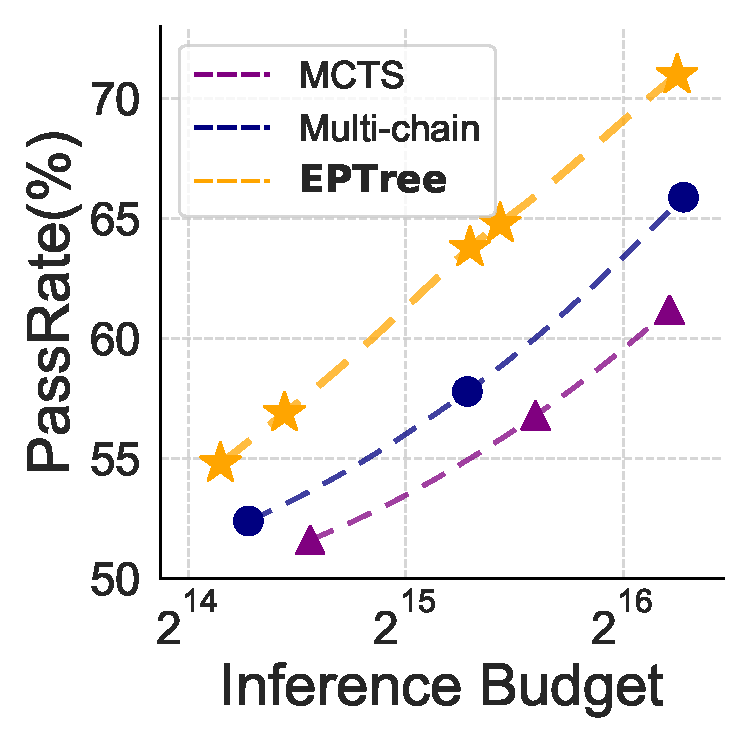
\includegraphics[width=\textwidth]{figure/head_tree_iid_mcts_performance.pdf}
        \label{fig:third_image}
    \vspace{-7mm}
    \end{minipage}
    \hfill
    \begin{minipage}{0.235\textwidth}
        \centering
        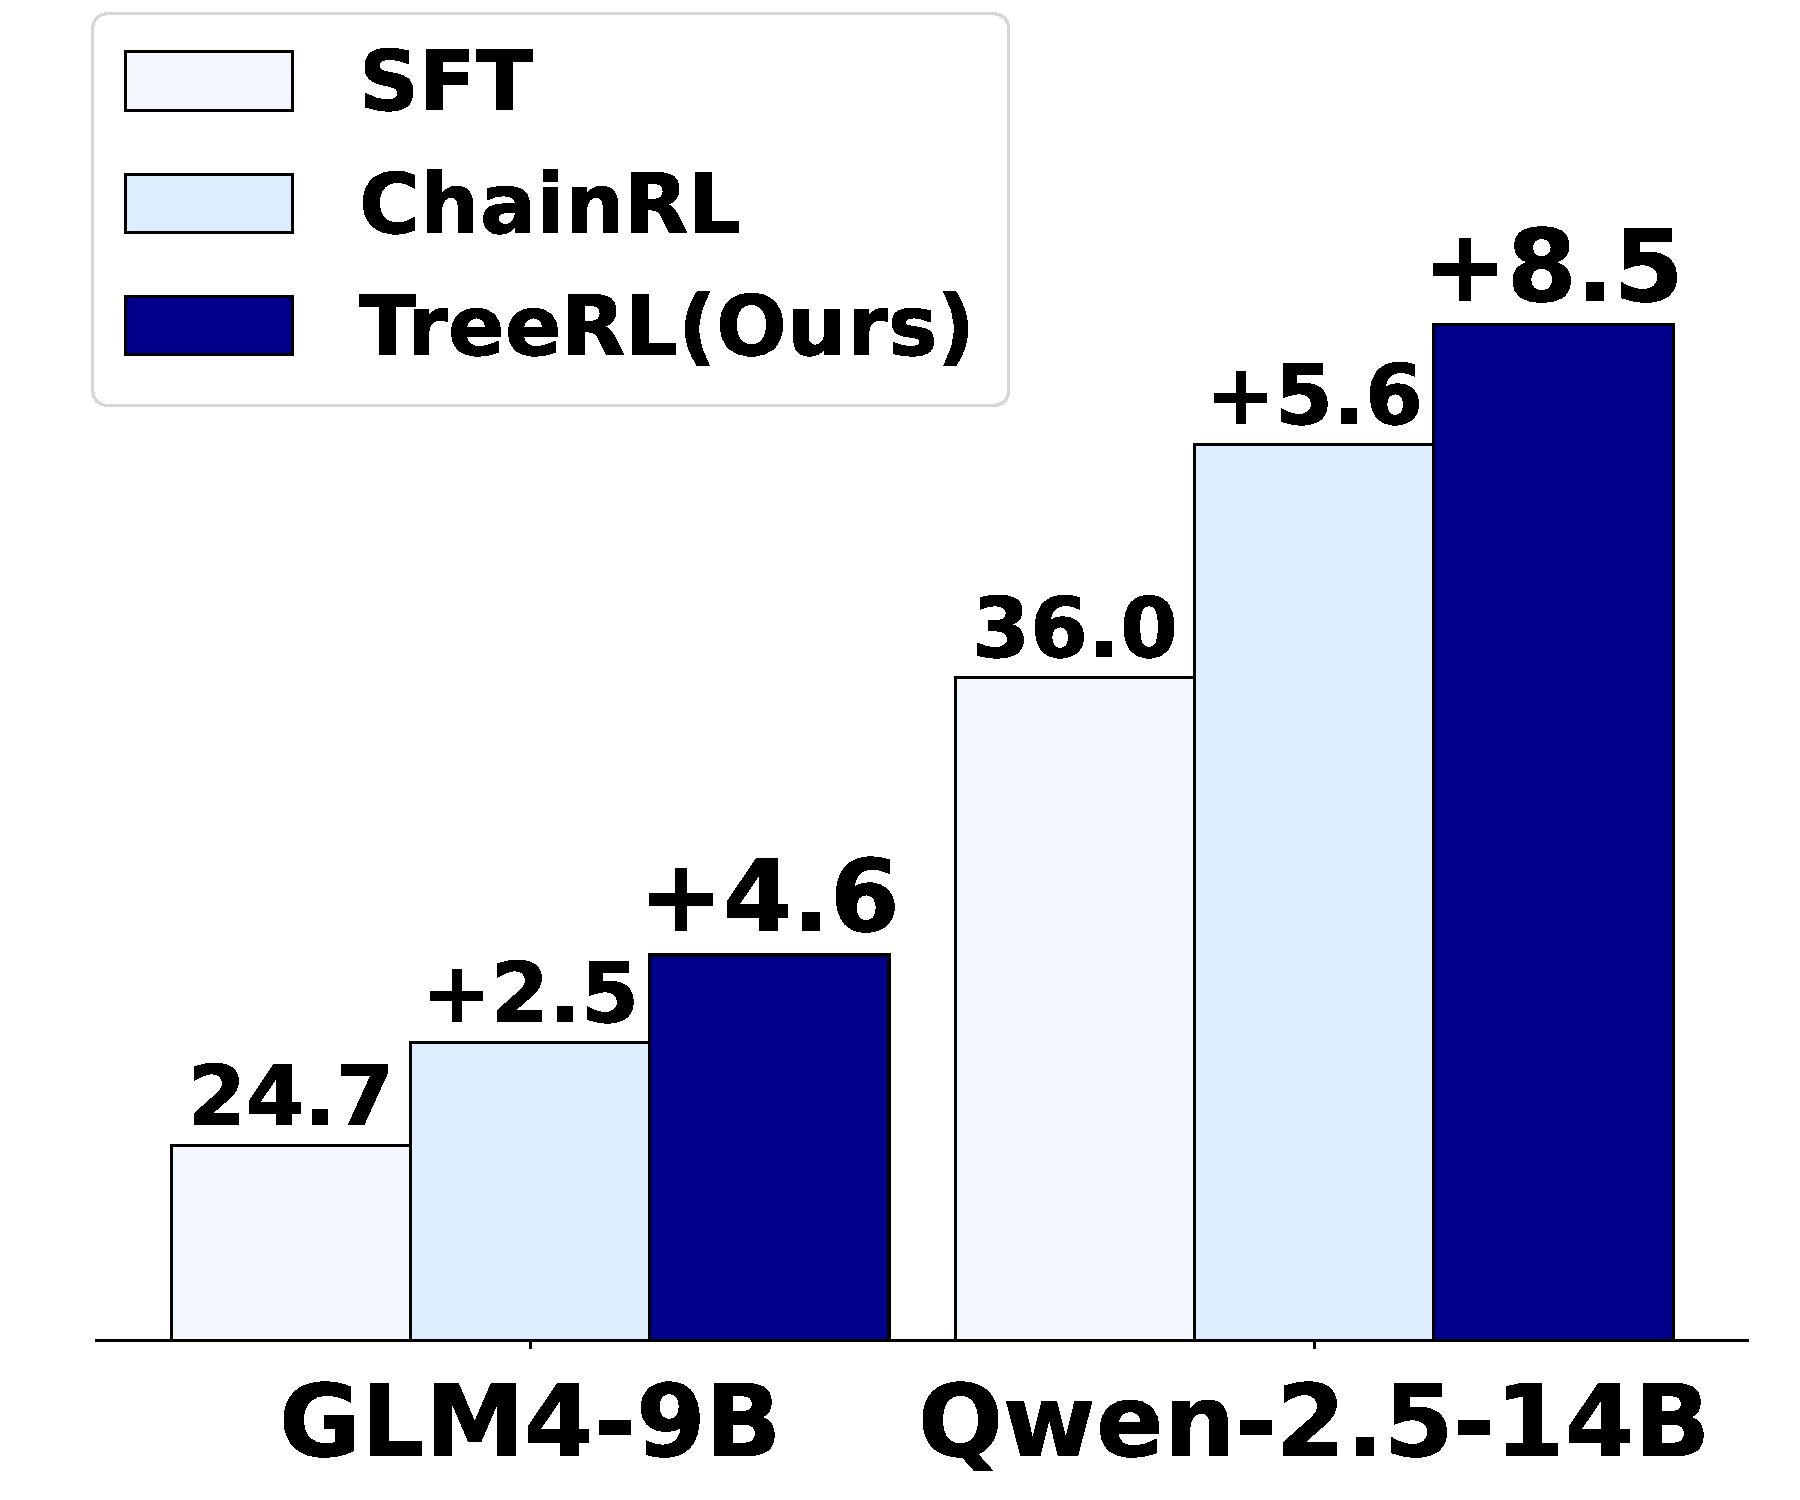
\includegraphics[width=\textwidth]{figure/performance-preview.pdf}
        \label{fig:third_image}
    \vspace{-3mm}
    \end{minipage}
    \vspace{-3mm}
    \caption{\textit{Left}: Performance comparison of sampling strategies. \treemodel consistently outperforms i.i.d multi-chain sampling and MCTS under different inference budgets. \textit{Right}: \model powered with \treemodel demonstrates better performance than ChainRL with i.i.d multi-chain sampling.}
    \label{fig:performance_preview}
\end{figure}


\begin{figure*}
    \centering
    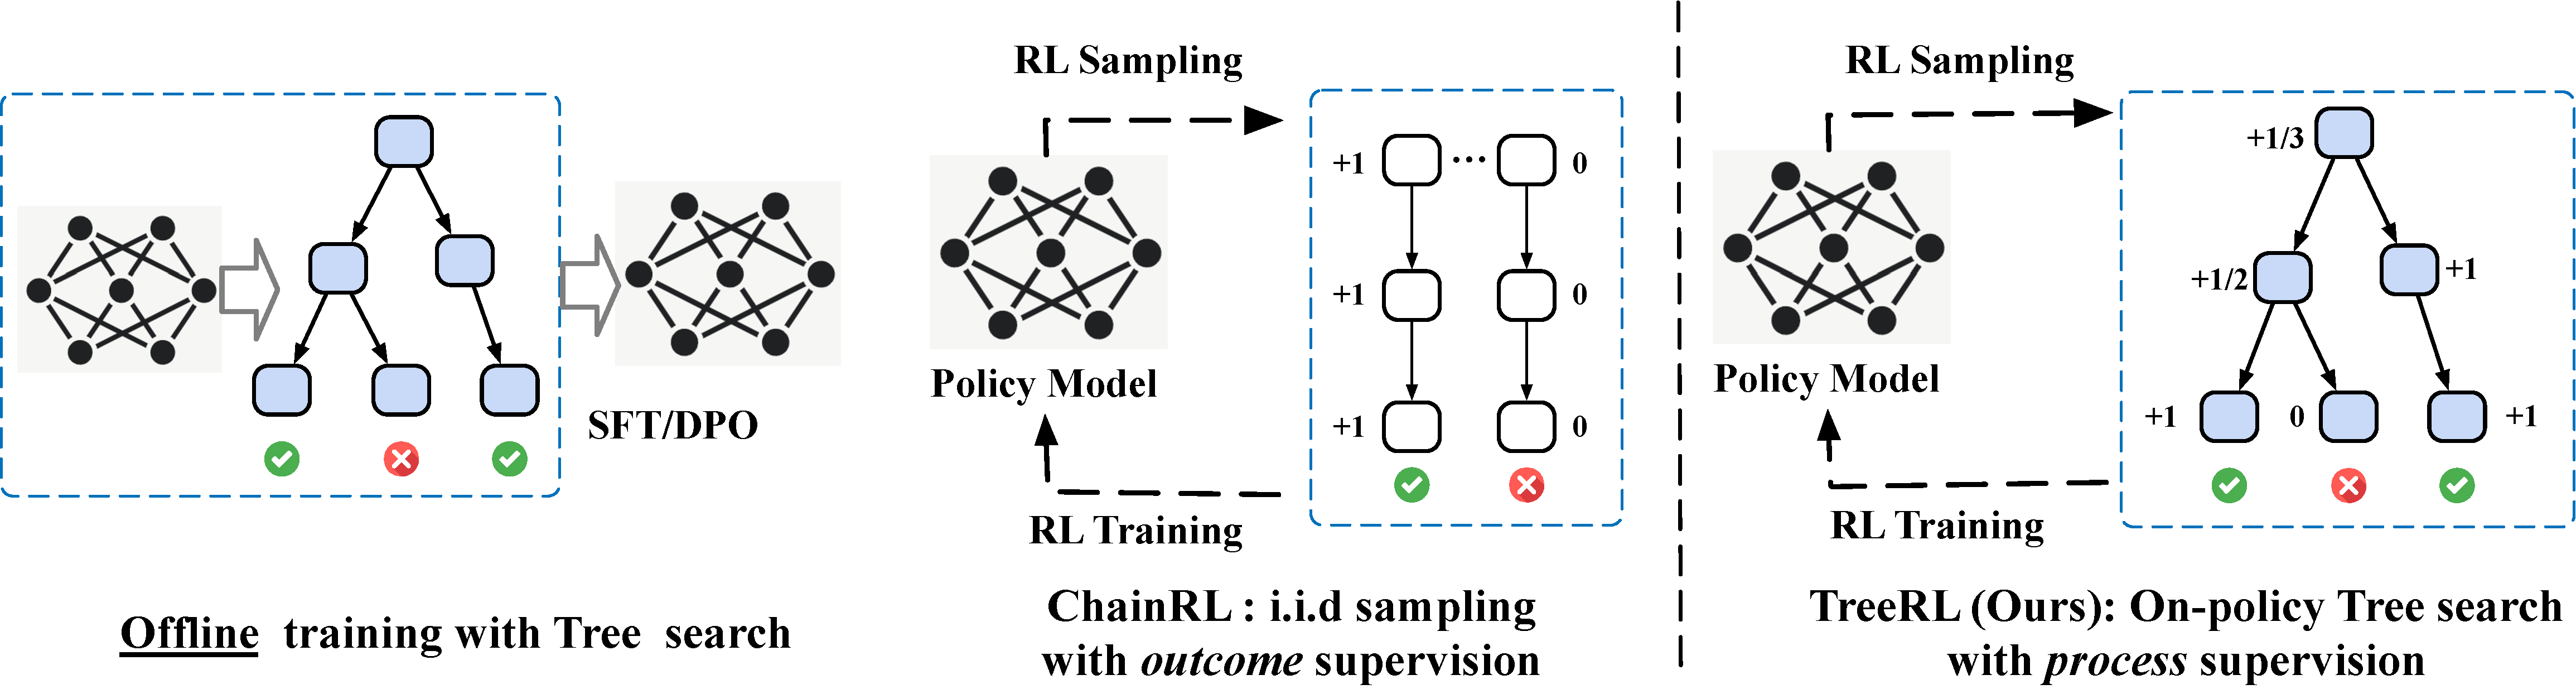
\includegraphics[width=\linewidth]{figure/illustration-v2.pdf}
    \caption{Illustration of offline training with tree search (Left), traditional ChainRL with online i.i.d multi-response sampling (Middle), and \model with tree search (Right).}
    \label{fig:illustration}
\end{figure*}


% \begin{table}[]
%     \centering
%     \begin{tabular}{lcc|c}
%     \toprule[1.2pt]
%          & Pass@$K$(\%) & Time(s) & \textit{w/} RL(\%) \\
%     \midrule
%         i.i.d chain & 52.0 & 35.5  \\
%         MCTS & 51.6 & 69.1 & \\
%         \treemodel (ours) & 56.9  & $55\sim 60$  \\
%     \bottomrule[1.2pt]
%     \end{tabular}
%     \caption{Performance comparison of i.i.d multi-chain sampling, MCTS, and the proposed \model under the same inference cost.}
%     \label{tab:my_label}
% \end{table}





Current RL methods for LLM training generally independently sample multiple trajectories~\cite{shao2024deepseekmath,wang2024mathshepherd,touvron2023llama2} and obtain reward signals based on the final answers. 
However, tree search, which has demonstrated significant success in other domains like AlphaZero~\cite{silver2017mastering}, remains under-developed in reinforcement learning for LLM reasoning. 
% Furthermore, tree search can provide fine-grained process-supervision signals~\citep{zhang2024rest,xie2024monte,luo2024autoimprove} rather than simply evaluating the entire trajectory solely on the final answer.
Existing efforts have mainly focused on using tree search to enhance inference-time performance alongside an external reward~\cite{zhang2024rest, chen2024alphamath}, or to produce data for offline training~\cite{chen2024alphamath,xie2024monte,zhang2024rest} (e.g., finetuning or DPO~\cite{rafailov2023direct}), as illustrated in Figure~\ref{fig:illustration}. But \citet{guo2025deepseek} also demonstrates the limitation of distribution shift and reward hacking in offline tree search compared to online RL training. Up to now, the potential of on-policy RL training incorporating tree search to improve LLM reasoning remains largely unexplored.


\hide{
The challenges are two-folds. First, classical Monte Carlo Tree Search (MCTS) can be less effective than independently sampling multiple responses under the same inference cost, which could hinder the performance of reinforcement learning. As shown in Table~\ref{fig:illustration}, MCTS exhibits worse PassRate performance and thus is less powerful in searching for the correct answer. 
Second, MCTS is far less efficient than sampling multiple responses because it demands numerous iterative, step-by-step generation, which suffers from lower parallel and is not friendly for the current LLM inference engine. 
}

\hide{
The challenges are two-fold. First, classical Monte Carlo Tree Search (MCTS)~\citep{browne2012mctssurvey} can be less effective than independently sampling multiple responses at the same inference cost, which can hinder the performance of reinforcement learning. As shown in Figure~\ref{fig:performance_preview}, MCTS demonstrates poorer PassRate performance, making it less effective in searching for the correct answer.
Second, MCTS is significantly less efficient than sampling multiple responses, as it requires numerous iterative, step-by-step generations. This process suffers from lower parallelism and is not well-suited for modern LLM inference engines.
}

The challenges are two-fold. First, classical Monte Carlo Tree Search (MCTS)~\citep{browne2012mctssurvey} can be less effective nd efficient than independently sampling multiple responses. MCTS achieves a lower PassRate performance under the same inference cost, as shown in Figure~\ref{fig:performance_preview}. The step-by-step generation requires numerous iterations and is not friendly to modern LLM inference engines.
Second, though tree search could provide fine-grained process supervision, the derived offline process reward model almost contributes to no performance improvement in RL training~\cite{guo2025deepseek}. 
% , which can hinder the performance of reinforcement learning. As shown in Figure~\ref{fig:performance_preview}, MCTS demonstrates poorer PassRate performance, making it less effective in searching for the correct answer.
% Second, MCTS is significantly less efficient than sampling multiple responses, as it requires numerous iterative, step-by-step generations. This process suffers from lower parallelism and is not well-suited for modern LLM inference engines.


% Tree search methods like Monte Carlo Tree Search (MCTS)~\cite{} can naturally provide process supervision signals. 
% However, they face two major challenges when applied to LLMs. First, MCTS is far less efficient than sampling multiple responses independently because it demands numerous iterative, step-by-step generation steps--a poor match for the current LLM inference paradigm. 
% Moreover, a large portion of these inference computations is effectively wasted and does not contribute to training, making MCTS a potential efficiency bottleneck. Second, as illustrated in Figure~\ref{fig:tree_vs_mcts_iid}, MCTS can be less effective in the LLM domain: under the same inference cost, MCTS exhibits worse Pass@$K$ performance than independent multiple sampling.

% There are two key drawbacks in the current RL training paradigm that merit improvement. First, most existing RL strategies~\cite{} for large language models (LLMs) evaluate the entire trajectory solely on the final answer. This practice assigns equal credit to every generation step, overlooking the distinct importance and potential of intermediate steps. To incorporate process supervision, prior works either employe a pretrained process reward model~\cite{}---which can be vulnerable to reward hacking---or relied on extensive Monte Carlo rollouts during training~\cite{}, which is computationally expensive ($O(n^2)$ complexity).

To address this gap, we propose \model, a reinforcement learning (RL) approach for LLMs employed with tree search. Under the same inference cost as independent multiple sampling, our method generates more diverse and effective responses and also provides on-policy process supervision signals to further boost RL performance.

First, we introduce an efficient and effective tree search strategy \treemodel.
Unlike MCTS which breaks answers into smaller parts to allow the model to explore step-by-step, we obtain a new response by forking branches from the most uncertain intermediate tokens in the existing tree based on entropy and continuing the generation until the final answer. Thus \treemodel requires fewer tokens but encourages effective exploration for the diverse answers.
And it typically requires only around two iterations to form the generation trees.

% To improve efficiency, we obtain a new response by selecting multiple intermediate tokens from an existing response and continuing the generation until the final answer. This approach is highly parallelizable and typically requires only two to three iterations to form the response trees. To improve effectiveness, we propose selecting tokens based on their uncertainty—measured by generation probability—and picking the top-M uncertain tokens for completion.

% One step further, we leverage the tree search to conduct reinforcement learning with process supervision signals. We assign credit to each generation step based on its advantage over other steps.
% The process signal of a reasoning step is defined as the weighted sum of 1) \emph{global advantage}: the advantage over the overall correct ratio for the question, and 2) \emph{local advantage}: the advantage over its parent step. Since the signals are derived from online-generated trees, they are not susceptible to reward hacking and do not rely on any additional reward models.

One step further, we leverage the tree search for reinforcement learning with process supervision. Each step in the trees is assigned a credit based on advantage, i.e., how much that step improves the likelihood of reaching a correct solution compared to other steps. The process signal for a given reasoning step is calculated as a weighted sum of two components: 1) global advantage, which reflects the step's potential over the overall correctness rate 
% across all generated solutions
for the question, and 2) local advantage, which quantifies the improvement the step provides compared to its parent step in the tree. Since these advantage signals are derived directly from the on-policy generated trees, they are inherently resistant to reward hacking~\citep{skalse2022defining} and do not rely on any additional reward models.

% initializing the value of each step as its probability of reaching the correct answer. 


We evaluate \model on challenging college-level and competition-level math and code reasoning benchmarks based on Qwen~\citep{qwen2_5} and GLM~\citep{glm2024chatglm}. Experiments show that \model achieves superior performance and demonstrates advantages over traditional independent multi-chain sampling. The gain benefits from both \treemodel with promising PassRate performance and process supervision. These results highlight the potential of RL with tree search to advance complex reasoning capabilities for LLM. The implementation of \model is available at \url{https://github.com/THUDM/TreeRL}. 



















\hide{
\section{Introduction}
Large language models (LLMs) have demonstrated remarkable capabilities across diverse complex reasoning tasks~\citep{achiam2023gpt,team2023gemini,dubey2024llama3}, including mathematics~\cite{shao2024deepseekmath}, programming~\citep{lozhkov2024starcoder,zhu2024deepseek}, and autonomous agents~\citep{zhouwebarena}.
% Reinforcement learning (RL) has emerged as a powerful tool to significantly boost LLM's reasoning ability, and enables models to optimize the policy through reward feedback
Reinforcement learning (RL) has emerged as a powerful approach to significantly improve the reasoning abilities of LLMs by optimizing the policy through reward feedback~\citep{openaio1,guo2025deepseek,hou2025advancing,shao2024deepseekmath}. 


\begin{figure}[t]
    \centering
    \begin{minipage}{0.235\textwidth}
        \centering
%        \includegraphics[width=\textwidth]{figure/tree_efficiency_preview.pdf}
        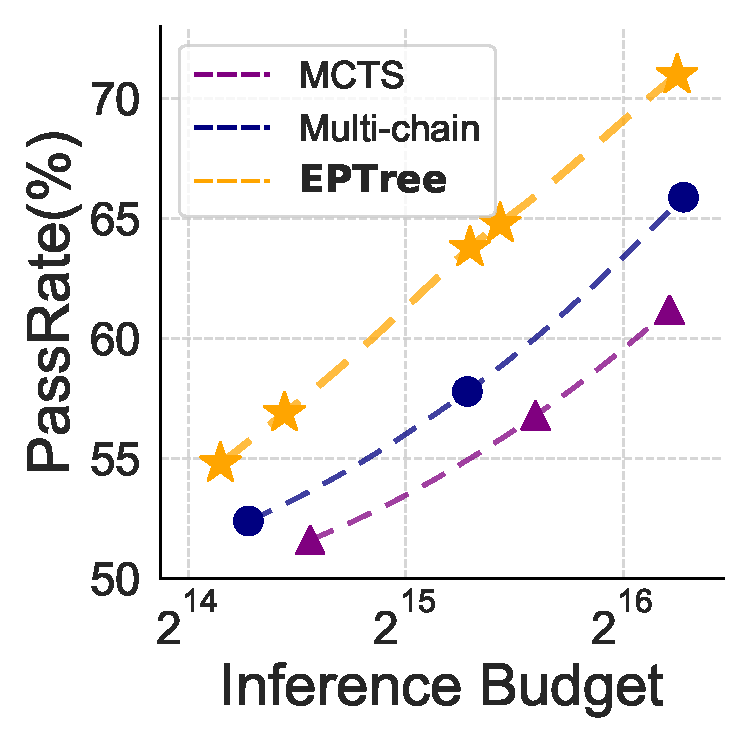
\includegraphics[width=\textwidth]{figure/head_tree_iid_mcts_performance.pdf}
        \label{fig:third_image}
    \vspace{-7mm}
    \end{minipage}
    \hfill
    \begin{minipage}{0.235\textwidth}
        \centering
        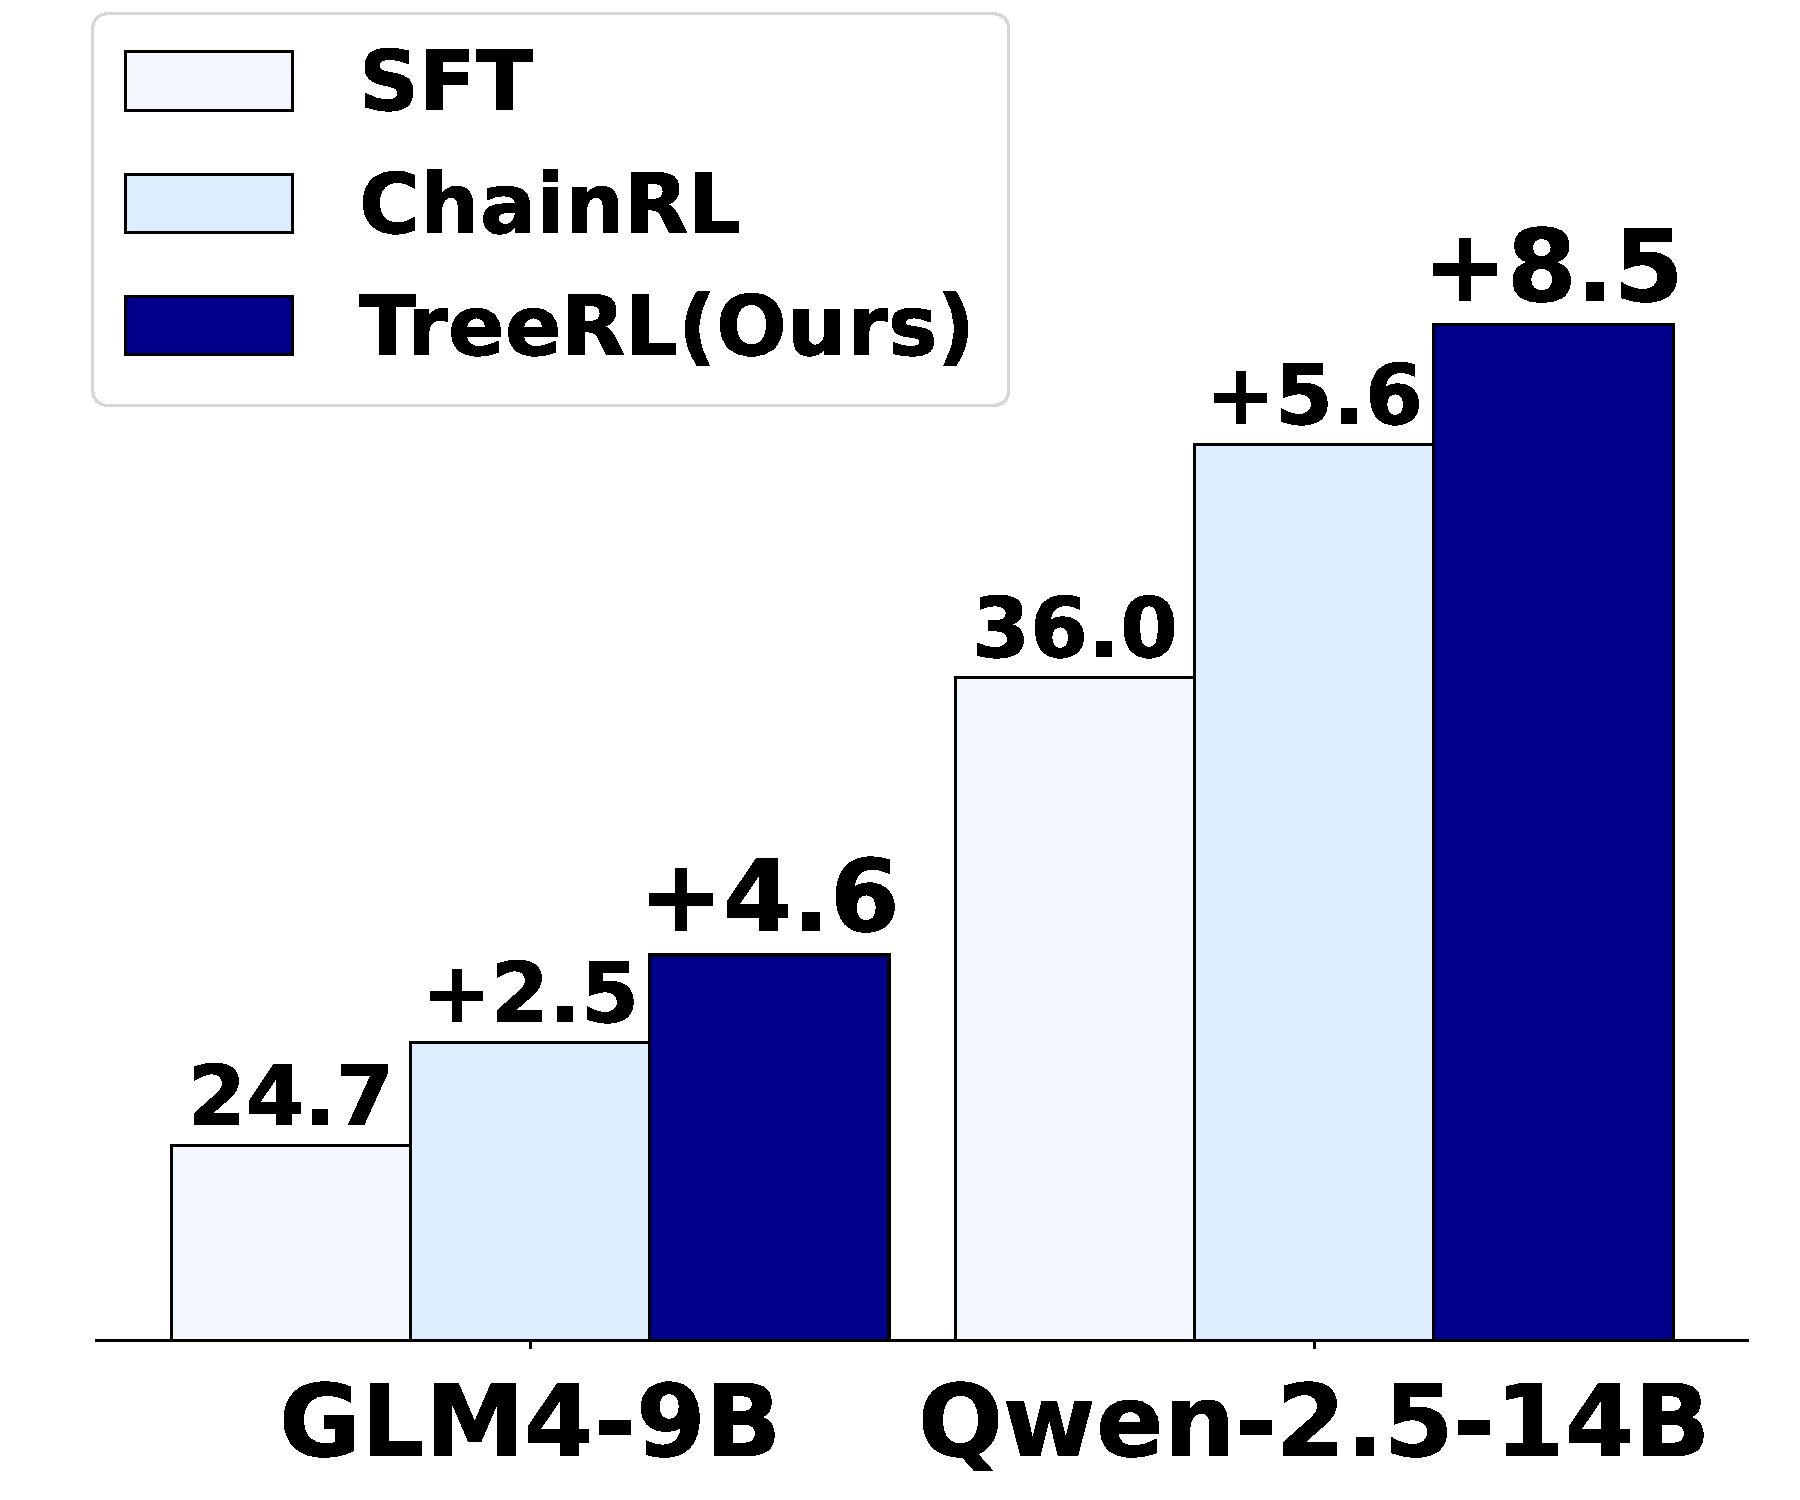
\includegraphics[width=\textwidth]{figure/performance-preview.pdf}
        \label{fig:third_image}
    \vspace{-3mm}
    \end{minipage}
    \vspace{-3mm}
    \caption{\textit{Left}: Performance comparison of sampling strategies. \treemodel consistently outperforms i.i.d multi-chain sampling and MCTS under different inference budgets. \textit{Right}: \model powered with \treemodel demonstrates better performance than ChainRL with i.i.d multi-chain sampling.}
    \label{fig:performance_preview}
\end{figure}


\begin{figure*}
    \centering
    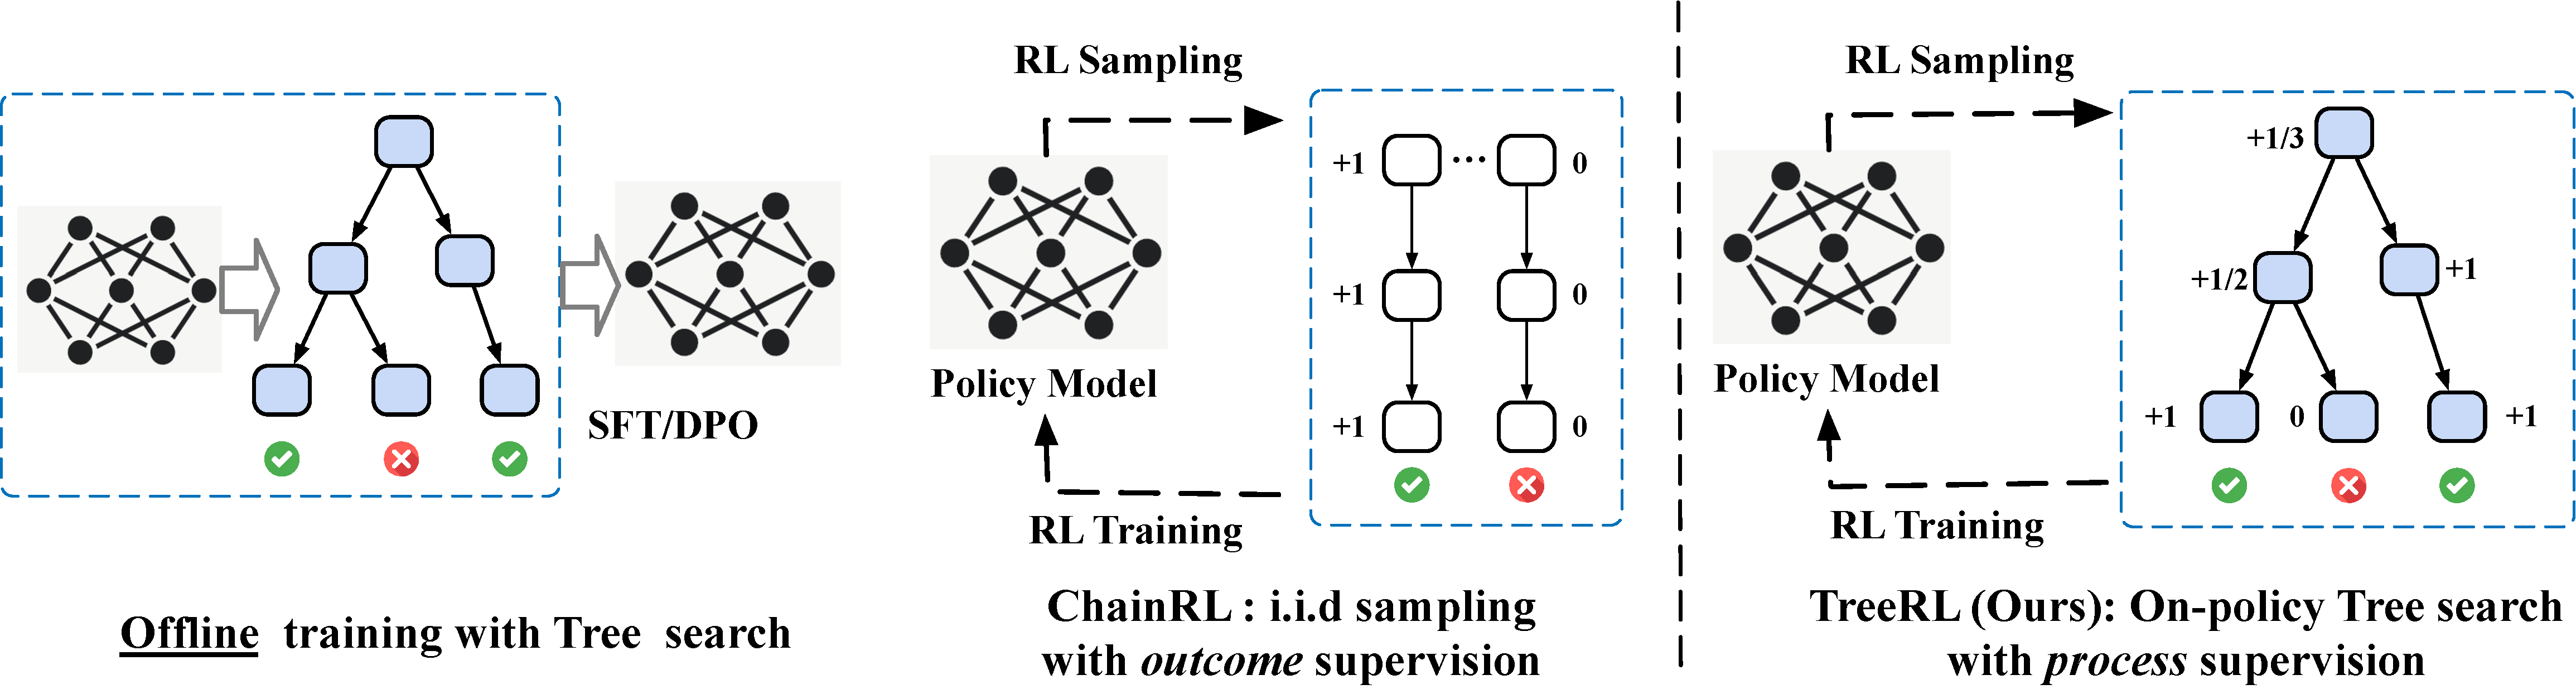
\includegraphics[width=\linewidth]{figure/illustration-v2.pdf}
    \caption{Illustration of offline training with tree search (Left), traditional ChainRL with online i.i.d multi-response sampling (Middle), and \model with tree search (Right).}
    \label{fig:illustration}
\end{figure*}


% \begin{table}[]
%     \centering
%     \begin{tabular}{lcc|c}
%     \toprule[1.2pt]
%          & Pass@$K$(\%) & Time(s) & \textit{w/} RL(\%) \\
%     \midrule
%         i.i.d chain & 52.0 & 35.5  \\
%         MCTS & 51.6 & 69.1 & \\
%         \treemodel (ours) & 56.9  & $55\sim 60$  \\
%     \bottomrule[1.2pt]
%     \end{tabular}
%     \caption{Performance comparison of i.i.d multi-chain sampling, MCTS, and the proposed \model under the same inference cost.}
%     \label{tab:my_label}
% \end{table}





Current RL methods for LLM training generally independently sample multiple trajectories~\cite{shao2024deepseekmath,wang2024mathshepherd,touvron2023llama2} and obtain reward signals based on the final answers. 
However, tree search, which has demonstrated significant success in other domains like AlphaZero~\cite{silver2017mastering}, remains under-developed in reinforcement learning for LLM reasoning. 
% Furthermore, tree search can provide fine-grained process-supervision signals~\citep{zhang2024rest,xie2024monte,luo2024autoimprove} rather than simply evaluating the entire trajectory solely on the final answer.
Existing efforts have mainly focused on using tree search to enhance inference-time performance alongside an external reward~\cite{zhang2024rest, chen2024alphamath}, or to produce data for offline training~\cite{chen2024alphamath,xie2024monte,zhang2024rest} (e.g., finetuning or DPO~\cite{rafailov2023direct}), as illustrated in Figure~\ref{fig:illustration}. But \citet{guo2025deepseek} also demonstrates the limitation of distribution shift and reward hacking in offline tree search compared to online RL training. Up to now, the potential of on-policy RL training incorporating tree search to improve LLM reasoning remains largely unexplored.


\hide{
The challenges are two-folds. First, classical Monte Carlo Tree Search (MCTS) can be less effective than independently sampling multiple responses under the same inference cost, which could hinder the performance of reinforcement learning. As shown in Table~\ref{fig:illustration}, MCTS exhibits worse PassRate performance and thus is less powerful in searching for the correct answer. 
Second, MCTS is far less efficient than sampling multiple responses because it demands numerous iterative, step-by-step generation, which suffers from lower parallel and is not friendly for the current LLM inference engine. 
}

\hide{
The challenges are two-fold. First, classical Monte Carlo Tree Search (MCTS)~\citep{browne2012mctssurvey} can be less effective than independently sampling multiple responses at the same inference cost, which can hinder the performance of reinforcement learning. As shown in Figure~\ref{fig:performance_preview}, MCTS demonstrates poorer PassRate performance, making it less effective in searching for the correct answer.
Second, MCTS is significantly less efficient than sampling multiple responses, as it requires numerous iterative, step-by-step generations. This process suffers from lower parallelism and is not well-suited for modern LLM inference engines.
}

The challenges are two-fold. First, classical Monte Carlo Tree Search (MCTS)~\citep{browne2012mctssurvey} can be less effective nd efficient than independently sampling multiple responses. MCTS achieves a lower PassRate performance under the same inference cost, as shown in Figure~\ref{fig:performance_preview}. The step-by-step generation requires numerous iterations and is not friendly to modern LLM inference engines.
Second, though tree search could provide fine-grained process supervision, the derived offline process reward model almost contributes to no performance improvement in RL training~\cite{guo2025deepseek}. 
% , which can hinder the performance of reinforcement learning. As shown in Figure~\ref{fig:performance_preview}, MCTS demonstrates poorer PassRate performance, making it less effective in searching for the correct answer.
% Second, MCTS is significantly less efficient than sampling multiple responses, as it requires numerous iterative, step-by-step generations. This process suffers from lower parallelism and is not well-suited for modern LLM inference engines.


% Tree search methods like Monte Carlo Tree Search (MCTS)~\cite{} can naturally provide process supervision signals. 
% However, they face two major challenges when applied to LLMs. First, MCTS is far less efficient than sampling multiple responses independently because it demands numerous iterative, step-by-step generation steps--a poor match for the current LLM inference paradigm. 
% Moreover, a large portion of these inference computations is effectively wasted and does not contribute to training, making MCTS a potential efficiency bottleneck. Second, as illustrated in Figure~\ref{fig:tree_vs_mcts_iid}, MCTS can be less effective in the LLM domain: under the same inference cost, MCTS exhibits worse Pass@$K$ performance than independent multiple sampling.

% There are two key drawbacks in the current RL training paradigm that merit improvement. First, most existing RL strategies~\cite{} for large language models (LLMs) evaluate the entire trajectory solely on the final answer. This practice assigns equal credit to every generation step, overlooking the distinct importance and potential of intermediate steps. To incorporate process supervision, prior works either employe a pretrained process reward model~\cite{}---which can be vulnerable to reward hacking---or relied on extensive Monte Carlo rollouts during training~\cite{}, which is computationally expensive ($O(n^2)$ complexity).

To address this gap, we propose \model, a reinforcement learning (RL) approach for LLMs employed with tree search. Under the same inference cost as independent multiple sampling, our method generates more diverse and effective responses and also provides on-policy process supervision signals to further boost RL performance.

First, we introduce an efficient and effective tree search strategy \treemodel.
Unlike MCTS which breaks answers into smaller parts to allow the model to explore step-by-step, we obtain a new response by forking branches from the most uncertain intermediate tokens in the existing tree based on entropy and continuing the generation until the final answer. Thus \treemodel requires fewer tokens but encourages effective exploration for the diverse answers.
And it typically requires only around two iterations to form the generation trees.

% To improve efficiency, we obtain a new response by selecting multiple intermediate tokens from an existing response and continuing the generation until the final answer. This approach is highly parallelizable and typically requires only two to three iterations to form the response trees. To improve effectiveness, we propose selecting tokens based on their uncertainty—measured by generation probability—and picking the top-M uncertain tokens for completion.

% One step further, we leverage the tree search to conduct reinforcement learning with process supervision signals. We assign credit to each generation step based on its advantage over other steps.
% The process signal of a reasoning step is defined as the weighted sum of 1) \emph{global advantage}: the advantage over the overall correct ratio for the question, and 2) \emph{local advantage}: the advantage over its parent step. Since the signals are derived from online-generated trees, they are not susceptible to reward hacking and do not rely on any additional reward models.

One step further, we leverage the tree search for reinforcement learning with process supervision. Each step in the trees is assigned a credit based on advantage, i.e., how much that step improves the likelihood of reaching a correct solution compared to other steps. The process signal for a given reasoning step is calculated as a weighted sum of two components: 1) global advantage, which reflects the step's potential over the overall correctness rate 
% across all generated solutions
for the question, and 2) local advantage, which quantifies the improvement the step provides compared to its parent step in the tree. Since these advantage signals are derived directly from the on-policy generated trees, they are inherently resistant to reward hacking~\citep{skalse2022defining} and do not rely on any additional reward models.

% initializing the value of each step as its probability of reaching the correct answer. 


We evaluate \model on challenging college-level and competition-level math and code reasoning benchmarks based on Qwen~\citep{qwen2_5} and GLM~\citep{glm2024chatglm}. Experiments show that \model achieves superior performance and demonstrates advantages over traditional independent multi-chain sampling. The gain benefits from both \treemodel with promising PassRate performance and process supervision. These results highlight the potential of RL with tree search to advance complex reasoning capabilities for LLM. The implementation of \model is available at \url{https://github.com/THUDM/TreeRL}. 

}